\noindent

\includegraphics[height=1.25cm]{images/pictograms/benchmark}

\includegraphics[height=1.25cm]{images/pictograms/FEM}

\includegraphics[height=1.25cm]{images/pictograms/paraview}

%%%%%%%%%%%%%%%%%%%%%%%%%%%%%%%%%%%%%%%%%%%%%%%%%%%%%%%%%%%%%%%%%%%%%%%%%%%%%%%%%%%%%%%%%%%%%%%%%%%

\begin{flushright} {\tiny {\color{gray} python\_codes/fieldstone\_76/text.tex}} \end{flushright}


\par\noindent\rule{\textwidth}{0.4pt}

\begin{center}
\inpython \hspace{0.5cm}
{\small Code: \url{https://github.com/cedrict/fieldstone/tree/master/python_codes/fieldstone_76}}
\end{center}

%\par\noindent\rule{\textwidth}{0.4pt}
%{\sl This stone was developed in collaboration with Donald Duck}. \index{contributors}{D. Duck}

\par\noindent\rule{\textwidth}{0.4pt}

Last revision: Feb. 15th, 2025.

\par\noindent\rule{\textwidth}{0.4pt}

%%%%%%%%%%%%%%%%%%%%%%%%%%%%%%%%%%%%%%%%%%%%%%%%%%%%%%%%%%%%%%%%%%%%%%%%%%%%%%%%%%%%%%%%%%%%%%%%%%%

%------------------------------------------------------------------------------
\subsection*{What the literature says}

According to \textcite{bobf08} 
{\color{darkgray} ``This element was apparently discovered 
around a blackboard at the Banff Conference on Finite Elements in 
Flow Problems (1979)''}.

\begin{center}
\begin{flushright} {\tiny {\color{gray} \tt (tikz\_p2pm1.tex)}} \end{flushright}
%~~~~~~~~~~~~~~~~~~~~~~~~~~~~~~~~~~~~~~~~~~~~~~~~~~~~~~~~~~~~~~~~~~~~~~~~~~~~~~~~~~~~~~~~~~~~~~~~~~


%\begin{center}
\begin{tikzpicture}
%\draw[fill=gray!23,gray!23](0,0) rectangle (5,5);
%\draw[step=0.5cm,gray,very thin] (0,0) grid (5,5); %background grid
\draw[thick] (1,1) -- (4,1) -- (4,3) -- (1,3) -- cycle;  
\node[] at (0.7,0.8) {0};
\node[] at (4.3,0.8) {1};
\node[] at (4.25,3.1) {2};
\node[] at (0.8,3.2) {3};
\draw[black,fill=teal] (1,1)     circle (2pt); 
\draw[black,fill=teal] (4,1)   circle (2pt); 
\draw[black,fill=teal] (4,3)   circle (2pt); 
\draw[black,fill=teal] (1,3) circle (2pt); 
\draw[black,fill=teal] (2.5,1) circle (2pt) ; 
\draw[black,fill=teal] (2.5,3) circle (2pt) ; 
\draw[black,fill=teal] (1,2) circle (2pt) ; 
\draw[black,fill=teal] (4,2) circle (2pt) ; 

\draw[violet] (2.5,2) circle (4pt);
\draw[violet] (3,2) circle (4pt);
\draw[violet] (2.5,2.5) circle (4pt);

\draw[black,fill=teal] (3.1,0.2) circle (2pt); 
\node[] at (3.4,0.2) {$\vec\upnu$};
\draw[violet] (4.1,0.2) circle (4pt); 
\node[] at (4.4,0.2) {$p$};
\node[] at (2.5,3.85) {9 vel. nodes, 3 press. nodes};
\end{tikzpicture}
%\end{center}

\end{center}

This element is crowned ``probably the most accurate 2D element'' in \textcite{grsa}.

It is characterised by piecewise bi/triquadratic velocities, 
and piecewise linear discontinuous polynomial pressure. 
The element satisfies the inf-sup condition, see p.~211 of \textcite{hugh}, or 
p.~138 of \textcite{elsw}.
It is used for example in \textcite{vavs89} (1989) for steady laminar flow in a curved tube
but also and more importantly it is the element pair used in \textcite{mabl15} (2015)
and it is available in \aspect too. 


When using this element one must be aware of the fact that there are 
two possible choices for the definitions of the pressure space 
(the so-called ``mapped'' and ``un-mapped'' variants) as explained
in \textcite{boga02} (2002). 

\textcite{bobf08} (2008) state: 
\begin{displayquote}
{\color{darkgray}
On a general quadrilateral mesh, the [pressure] space 
can be defined in two different ways: either [it] 
consists of (discontinuous) piecewise linear functions, or it is built
by considering three linear shape functions on the reference unit square and mapping
them to the general elements like it is usually done for continuous 
finite elements. [...] We shall refer to the first possibility as 
unmapped pressure approach and to the second one as mapped pressure approach.

[...] 

So far, we have shown that either the 
unmapped and the mapped pressure 
approach gives rise to a stable ${\bm Q}_2\times P_{-1}$ scheme. 
However, as a consequence of the
results proved in \textcite{arbf02} (2002), we have that the mapped 
pressure approach cannot achieve 
optimal approximation order. Namely, the unmapped pressure space 
provides a second-order convergence 
in $L_2$, while the mapped one achieves only ${\cal O}(h)$ in the same norm.}
\end{displayquote}

We also read in \textcite{boga02} (2002):
\begin{displayquote}
{\color{darkgray}
Two possible choices are given for the definition of the pressure space: 
one can either use a global pressure approximation (that is on
each quadrilateral the finite element space is spanned by 1 and by the 
global co-ordinates $x$ and $y$) or a local approach (consisting in generating 
the local space by means of the constants and the local curvilinear 
co-ordinates on each quadrilateral $r$ and $s$). [...] Numerical results 
actually show that the second choice (local or mapped pressure approximation) 
is suboptimally convergent.
}
\end{displayquote}



See also discussion about mapped/unmapped in \textcite{bobf13} and 
in Section 3.6.4 of \textcite{john16}.

This element is mentioned in \textcite{kaus10} (2010) and \textcite{pefc89} (1989) 
and it is used in \textcite{freh14} (2014) to study 3D fold growth rates 
(see online supplementary material) and in \textcite{schm08} (2008).

Note that the serendipity version of this pair, 
i.e. ${\bm Q}_2^{(20)}\times P_{-1}$ is also LBB stable
as shown in p180 of Reddy \cite{reddybook2}.

{\color{red} since I wrote this I have purchased many relevant FE books
and I need to go through all and extract relevant facts and remarks about 
this element pair.}


%------------------------------------------------------------------------------
\subsection*{Deriving the mapped vs un-mapped pressure basis functions}

The mapped version consists of  
using the $P_{-1}$ basis functions defined in Section~\ref{MMM-ss:lbfq2D}:
inside the reference element the pressure is given by $p^h(r,s)=a+br+cs$.
The reference element is the $[-1:1]^2$ square in the 2d Cartesian axis
system $r,s$.
Nodes are placed as follows: node 0 at (0,0), node 1 at (1,0) and node 2 at (0,1).
This yields the following basis functions
\begin{align}
\bN_0^p &= 1-r-s \nn\\
\bN_1^p &= r \nn\\
\bN_2^p &= s \nn
\end{align}
with 
\[
p^h(r,s) = \sum_{k=0}^2 \bN_k^p(r,s) \ p_k
\]
Obviously we recover $\sum_k \bN_k^p = 1$ and $\bN_k^p(r_i,s_i)=\delta_{ik}$.


The un-mapped version is a bit less straightforward and is as follows:
let us assume there are three distinct pressure nodes inside the element.
Inside each element the pressure is defined by a linear field
\[
p^h(x,y) = a+bx+cy
\]
We must then compute the coefficients $a,b,c$. We know that 
the expression above evaluated at the pressure nodes with 
coordinates $(x_i,y_i)$ should be equal to $p_i$. 
Then we have the following three equations:
\begin{eqnarray}
a + bx_1 + cy_1 &=& p_0 \nn\\
a + bx_2 + cy_2 &=& p_1 \nn\\
a + bx_3 + cy_3 &=& p_2 \nn
\end{eqnarray}
or, 
\[
\left(
\begin{array}{ccc}
1 & x_1 & y_1 \\
1 & x_2 & y_2 \\
1 & x_3 & y_3 
\end{array}
\right)
\cdot 
\left(
\begin{array}{ccc}
a \\ b \\ c
\end{array}
\right)
=
\left(
\begin{array}{ccc}
p_0 \\ p_1 \\ p_2
\end{array}
\right)
\]
Then 
\[
\left(
\begin{array}{ccc}
a \\ b \\ c
\end{array}
\right)
=
\left(
\begin{array}{ccc}
1 & x_1 & y_1 \\
1 & x_2 & y_2 \\
1 & x_3 & y_3 
\end{array}
\right)^{-1}
\cdot
\left(
\begin{array}{ccc}
p_0 \\ p_1 \\ p_2
\end{array}
\right)
= {\bm M}^{-1} \cdot \vec{p}
\]
with 
\[
{\bm M}^{-1} = \frac{1}{\Delta}
\left(
\begin{array}{ccc}
x_2y_3-x_3y_2 & x_3y_1-x_1y_3 & x_1y_2-x_2y_1 \\
y_2-y_3 & y_3-y_1 & y_1-y_2 \\
x_3-x_2 & x_1-x_3 & x_2-x_1
\end{array}
\right)
=
\left(
\begin{array}{ccc}
m_{11} & m_{12} & m_{13} \\
m_{21} & m_{22} & m_{23} \\
m_{31} & m_{32} & m_{33} 
\end{array}
\right)
\]
and
\[
\Delta = x_2y_3-x_3y_2 - x_1y_3-x_3y_1 + x_1y_2-x_2y_1
\]
so that
\begin{eqnarray}
a &=& m_{11}p_0 + m_{12} p_1 + m_{13} p_2 \nn\\
b &=& m_{21}p_0 + m_{22} p_1 + m_{23} p_2 \nn\\
c &=& m_{31}p_0 + m_{32} p_1 + m_{33} p_2 \nn
\end{eqnarray}
In the end 
\begin{eqnarray}
p^h(x,y) 
&=&  a+bx+cy \nn\\
&=& m_{11}p_0 + m_{12} p_1 + m_{13} p_2
+ ( m_{21}p_0 + m_{22} p_1 + m_{23} p_2) x
+ ( m_{31}p_0 + m_{32} p_1 + m_{33} p_2) y \nn\\
&=& \underbrace{(m_{11} + m_{21}x + m_{31}y)}_{\bN_0^p(x,y)} p_0 
+   \underbrace{(m_{12} + m_{22}x + m_{32}y)}_{\bN_1^p(x,y)} p_1 
+   \underbrace{(m_{13} + m_{23}x + m_{33}y)}_{\bN_1^p(x,y)} p_2
\label{f76_NNNP}
\end{eqnarray}
The basis functions are then evaluated at the (real) coordinates 
of the quadrature point $(x_q,y_q)$.

{\color{red} Q1: is this the right/standard way of deriving these 
basis functions? I suspect not. How is this carried out in deal.II?}





%------------------------------------------------------------------------------
\subsection*{About the code}


The 2d $Q_2$ shape functions have been derived in Section~\ref{MMM-ss:q22d}.
%The $-1$ subscript indicates that the pressure field is linear (but not bilinear!)
%as explained in Section~\ref{MMM-ss:pairq2pm1}.

For all the tests/benchmarks the box is a unit square.
Velocity nodes coordinates are stored in the \lstinline{xV,yV} arrays
with the \lstinline{iconV} connectivity array.
Pressure nodes coordinates are stored in the \lstinline{xP,yP} arrays
with the \lstinline{iconP} connectivity array.

The mesh counts \lstinline{nel=nelx*nely} elements,
\lstinline{NV=(2*nelx+1)*(2*nely+1)} velocity nodes and 
\lstinline{NP=3*nel} pressure nodes.

The \lstinline{meth} parameter is 1 for mapped approach and 2 
for un-mapped approach. 

I have implemented three different types of meshes. 
The first type is straightforward: all elements are rectangular (and in 
practice square for simplicity).

The second type sees a random perturbation added to interior nodes.
The parameter \lstinline{xi} controls the randomness of the mesh as follows:
for each node inside the domain (i.e. not on the boundaries) a random value 
in the range $[-\xi,\xi]$ ($\xi$ is set to 0.1 by default) 
is added to the $x$ and $y$ coordonates:
\begin{lstlisting}
for i in range(0,NV):
    if xV[i]>0 and xV[i]<Lx and yV[i]>0 and yV[i]<Ly:
       xV[i]+=random.uniform(-1.,+1)*hx*xi
       yV[i]+=random.uniform(-1.,+1)*hy*xi
\end{lstlisting}

The third type is as follows: it is borrowed from \stone~25 which models the 
Rayleigh-Taylor experiment of \textcite{vaks97} (1997). Only the vertical position 
of the nodes is modified: nodes at about 1/5 the height of the domain are set to 
follow a sinusoidal perturbation and the position of other nodes above or below
is then adjusted. See figure below. 

The internal numbering of velocity nodes is as follows:
\begin{verbatim}
3--6--2
|     |
7  8  5
|     |
0--4--1
\end{verbatim}

Very importantly, when mesh randomization or mesh deformation is used 
I make sure that the velocity nodes 4,5,6,7 in the middle of the edges 
are really put back between nodes 0-1, 1-2, 2-3, and 3-0 respectively. 
The node in the middle of the element is also then moved accordingly.
\begin{lstlisting}
for iel in range(0,nel):
    xV[iconV[4,iel]]=0.5*(xV[iconV[0,iel]]+xV[iconV[1,iel]])
    yV[iconV[4,iel]]=0.5*(yV[iconV[0,iel]]+yV[iconV[1,iel]])
    xV[iconV[5,iel]]=0.5*(xV[iconV[1,iel]]+xV[iconV[2,iel]])
    yV[iconV[5,iel]]=0.5*(yV[iconV[1,iel]]+yV[iconV[2,iel]])
    xV[iconV[6,iel]]=0.5*(xV[iconV[2,iel]]+xV[iconV[3,iel]])
    yV[iconV[6,iel]]=0.5*(yV[iconV[2,iel]]+yV[iconV[3,iel]])
    xV[iconV[7,iel]]=0.5*(xV[iconV[3,iel]]+xV[iconV[0,iel]])
    yV[iconV[7,iel]]=0.5*(yV[iconV[3,iel]]+yV[iconV[0,iel]])
    xV[iconV[8,iel]]=0.25*(xV[iconV[0,iel]]+xV[iconV[1,iel]]+xV[iconV[2,iel]]+xV[iconV[3,iel]])
    yV[iconV[8,iel]]=0.25*(yV[iconV[0,iel]]+yV[iconV[1,iel]]+yV[iconV[2,iel]]+yV[iconV[3,iel]])
\end{lstlisting}

The three types of meshes are shown here:

\begin{center}
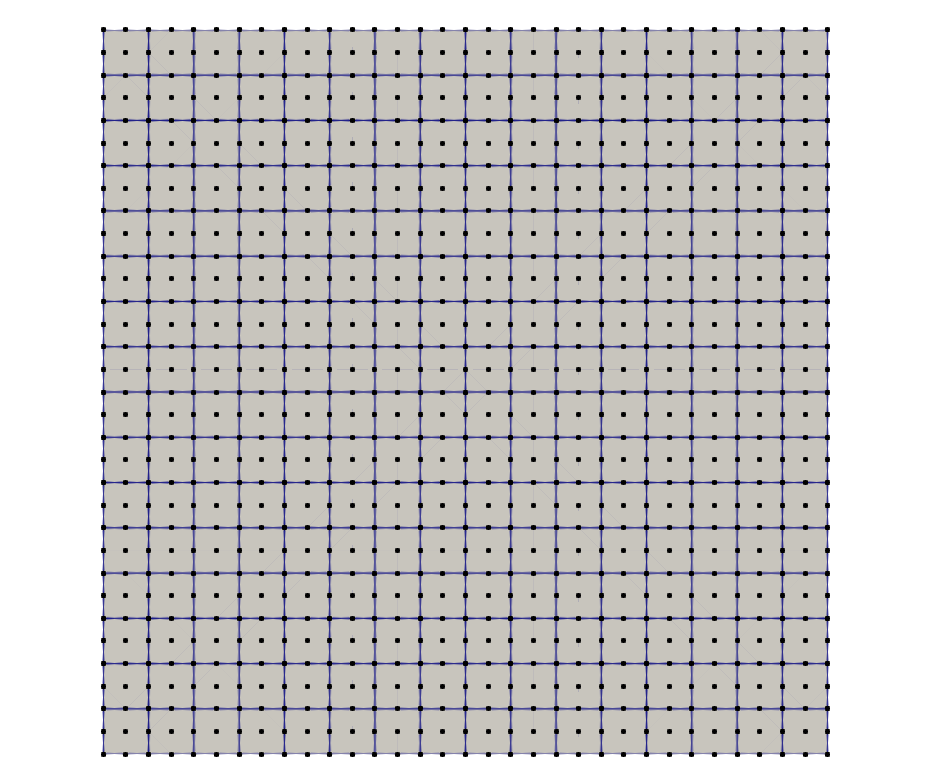
\includegraphics[width=5.7cm]{python_codes/fieldstone_76/results/mesh_type1}
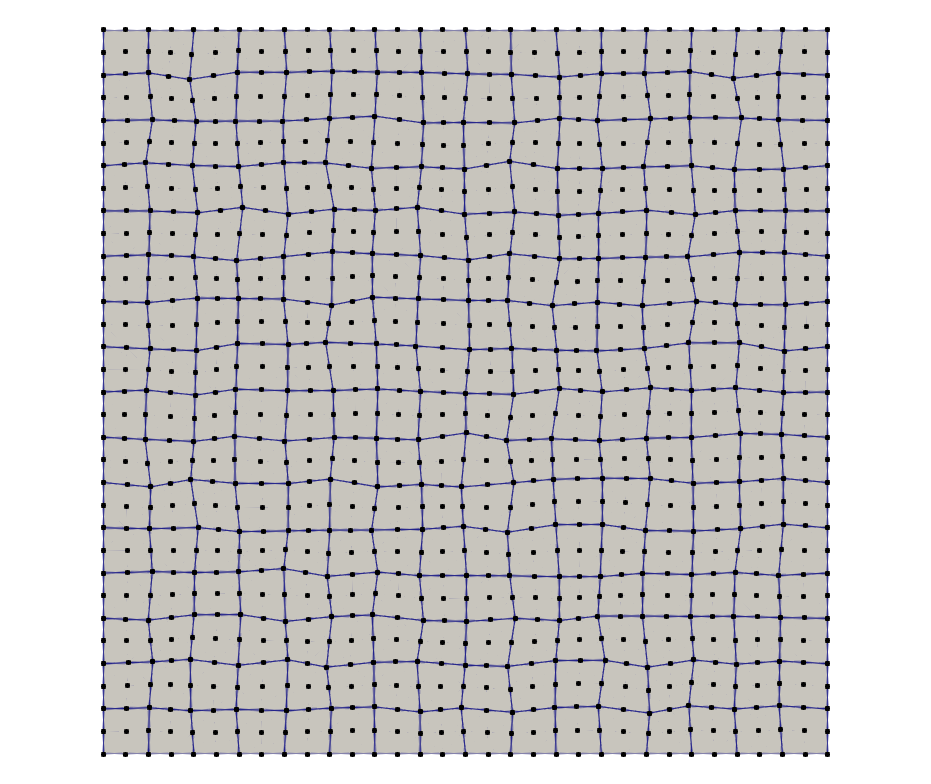
\includegraphics[width=5.7cm]{python_codes/fieldstone_76/results/mesh_type2}
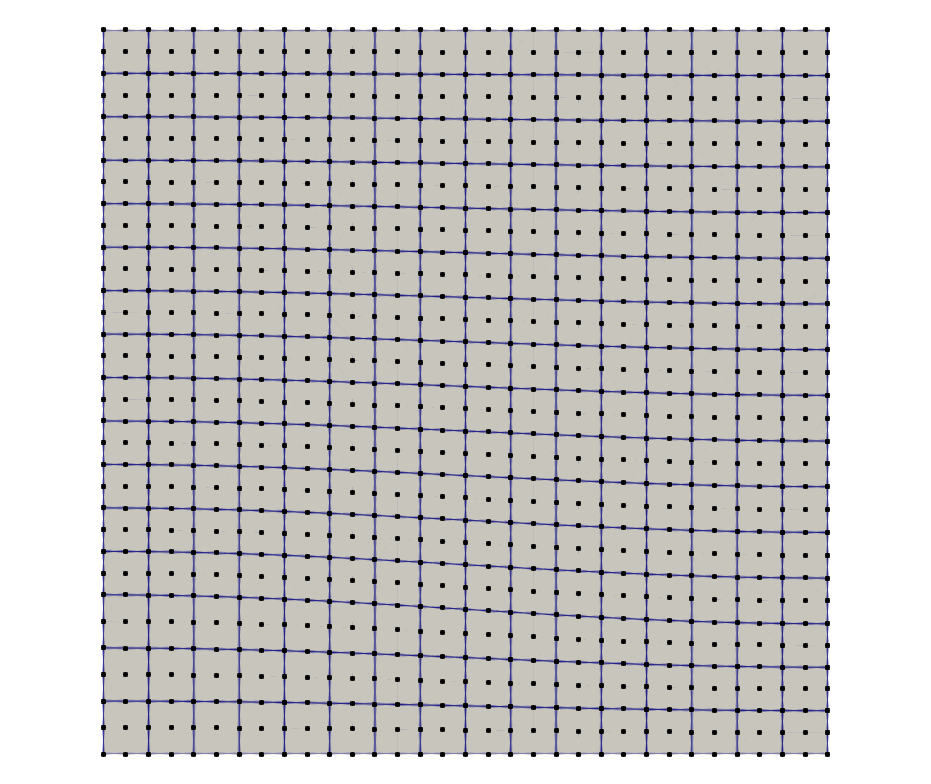
\includegraphics[width=5.7cm]{python_codes/fieldstone_76/results/mesh_type3}\\
{\captionfont From left to right: mesh types 1, 2, and 3, or 'square', 'random' 
and 'wave' meshes. Elements on the left are squares. Elements on the right are trapezes (their
vertical edges are parallel).}
\end{center}

Looking at the meshes above we find that the elements of the 'wave' mesh 
can be obtained by affine transformation\footnote{\url{https://en.wikipedia.org/wiki/Affine_transformation}} 
of the reference element but not the elements of the 'random' mesh. 
Quickly: an affine transformation 
is a geometric transformation that preserves lines and parallelism, but not necessarily 
Euclidean distances and angles. 
I remember coming across this terminology in the relevant literature (which I need to find again!)
and this may explain the results obtained for the manufactured solutions I ran the code on 
in what follows on both these types of meshes.

The mapping is isoparametric (i.e. $Q_2$). The same mapping is used for all integrals.
In the case of rectangular elements both the mapped and un-mapped approaches 
yield the same pressure basis functions values at the quadrature points
so the measured errors and vrms are identical.
{\color{red} Q2: I guess this is true for all elements obtained by affine transformation
from reference element?} 

The same quadrature rule is used for $\K$ and $\G$ blocks (called $A$ and $B$ blocks respectively in the
ASPECT literature).
I explore the effect of the number of quadrature points on the solution, 
so I allow for $2^2$, $3^2$ and $4^2$ quadrature points
as parameterized by the \lstinline{nqperdim} parameter.
Note that a $2^2$ is not sufficient to exactly integrate the 
terms found in the $\K$ and $\G$ blocks, $3^2$ is standard, 
and $4^2$ is probably overkill.

One source of uncertainty on my part is how/where to setup the pressure nodes.
For mapped elements the $P_{-1}$ pressure basis functions are defined as 
\begin{lstlisting}
def NNP(r,s):
    NP_0=1-r-s
    NP_1=r
    NP_2=s
    return np.array([NP_0,NP_1,NP_2],dtype=np.float64)
\end{lstlisting}
In other words the first pressure node is at coordinates $(0,0)$,
the second at $(1,0)$ and the third at $(0,1)$ inside the reference element $(r,s)\in[-1,+1]^2$
as shown here:

\begin{verbatim}
3--6--2   +--2--+
|     |   |     |
7  8  5   +  0  1
|     |   |     |
0--4--1   +--+--+

V nodes   P nodes
\end{verbatim}


For the un-mapped version we need to define the pressure node coordinates 
directly in the $(x,y)$ coordinates.
At the moment it is done as follows: The ninth velocity node of the element is 
in the center of the element and is also the first pressure node.
Since the elements are marginally deformed I can place the second pressure node 
a distance $h_x/2$ in the $x$-direction from the first point, and the third pressure node 
a distance $h_y/2$ in the $y$-direction from the first point.

\begin{lstlisting}
counter=0
for iel in range(nel):
    xP[counter]=xV[iconV[8,iel]]
    yP[counter]=yV[iconV[8,iel]]
    counter+=1
    xP[counter]=xV[iconV[8,iel]]+hx/2
    yP[counter]=yV[iconV[8,iel]]
    counter+=1
    xP[counter]=xV[iconV[8,iel]]
    yP[counter]=yV[iconV[8,iel]]+hy/2
    counter+=1
\end{lstlisting}
In this case the pressure basis functions need to be computed
element by element following Eq.~\eqref{f76_NNNP}:

\begin{lstlisting}
for iel in range(0,nel):
    if meth==2:
       det=xP[iconP[1,iel]]*yP[iconP[2,iel]]-xP[iconP[2,iel]]*yP[iconP[1,iel]]\
          -xP[iconP[0,iel]]*yP[iconP[2,iel]]+xP[iconP[2,iel]]*yP[iconP[0,iel]]\
          +xP[iconP[0,iel]]*yP[iconP[1,iel]]-xP[iconP[1,iel]]*yP[iconP[0,iel]]
       m11=(xP[iconP[1,iel]]*yP[iconP[2,iel]]-xP[iconP[2,iel]]*yP[iconP[1,iel]])/det
       m12=(xP[iconP[2,iel]]*yP[iconP[0,iel]]-xP[iconP[0,iel]]*yP[iconP[2,iel]])/det
       m13=(xP[iconP[0,iel]]*yP[iconP[1,iel]]-xP[iconP[1,iel]]*yP[iconP[0,iel]])/det
       m21=(yP[iconP[1,iel]]-yP[iconP[2,iel]])/det
       m22=(yP[iconP[2,iel]]-yP[iconP[0,iel]])/det
       m23=(yP[iconP[0,iel]]-yP[iconP[1,iel]])/det
       m31=(xP[iconP[2,iel]]-xP[iconP[1,iel]])/det
       m32=(xP[iconP[0,iel]]-xP[iconP[2,iel]])/det
       m33=(xP[iconP[1,iel]]-xP[iconP[0,iel]])/det
\end{lstlisting}


{\color{red} Q3: In the near future I want to try elements that 
showcase curves edges (esp. for the wave mesh). How am I then to place the 
velocity node in the 'middle' and the pressure nodes ??}

In both cases (mapped and un-mapped) the pressure is discontinuous from an element to another 
and this adds complexity in terms of exporting it to vtu format (and plotting with paraview). 
I then simply choose to export the value of the pressure in the middle of 
each element\footnote{I should improve this in the future, but it is 
only a visualisation problem and does not influence results.}

Quick summary of what follows without going into 
much detail: I carry out three benchmarks based on manufactured solutions  
and recover the expected cubic convergence for the velocity error 
and a quadratic error convergence for the pressure 
\textit{only} for the un-mapped approach.
Quadratic pressure error convergence is obtained with mapped elements 
only on square and wave meshes, with a linear convergence for random meshes. 



\newpage
%.......................................................
\subsection*{Manufactured solution of Donea \& Huerta ({\tt bench=3})}

This is the Donea \& Huerta benchmark that is fully described in Section~\ref{MMM-mms1}.

\begin{eqnarray}
u(x,y) &=& x^2(1-x)^2 2y (y-1)(2y-1) \nonumber\\
v(x,y) &=& -y^2 (1 - y)^2 2x (x-1)(2x-1) \nonumber\\
p(x,y) &=& x(1 -x)- 1/6 \nonumber 
\end{eqnarray}
Note that the pressure obeys $\int_{\Omega} p \; dV = 0$.


\begin{center}
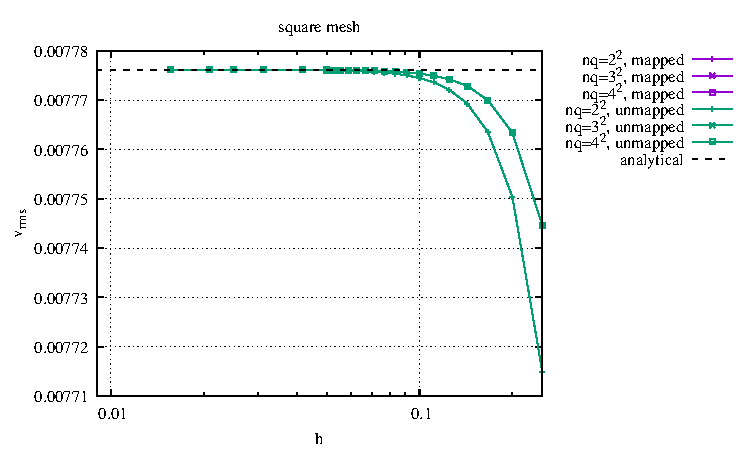
\includegraphics[width=5.7cm]{python_codes/fieldstone_76/results/bench3/reg/vrms}
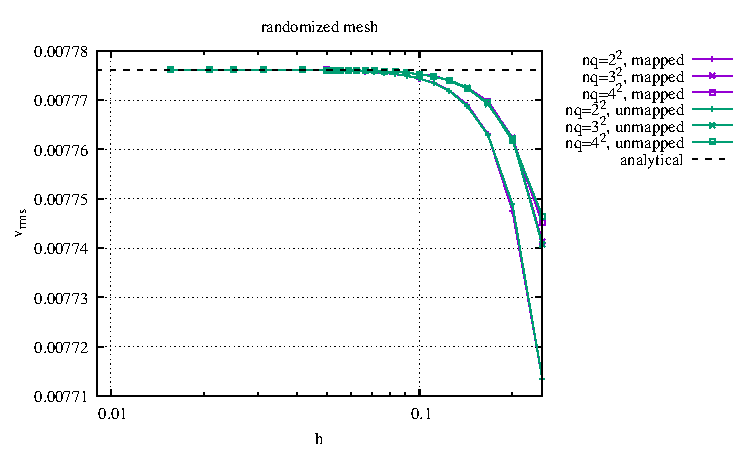
\includegraphics[width=5.7cm]{python_codes/fieldstone_76/results/bench3/rand/vrms}
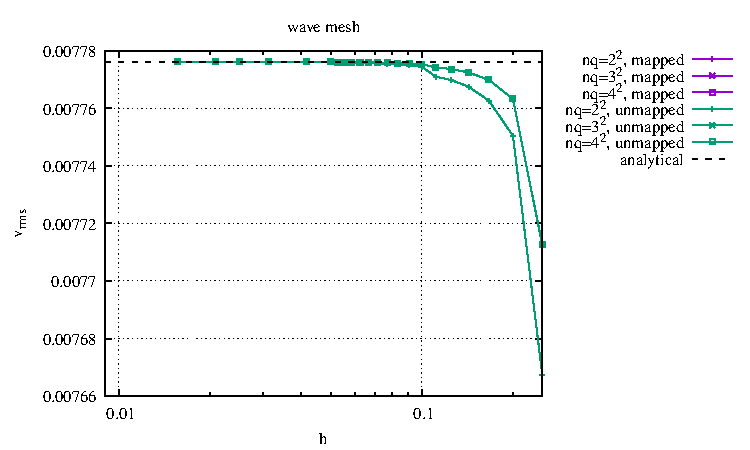
\includegraphics[width=5.7cm]{python_codes/fieldstone_76/results/bench3/wave/vrms}\\
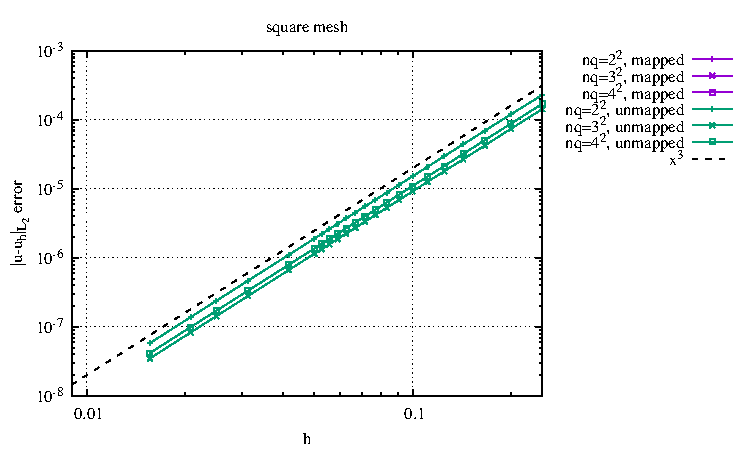
\includegraphics[width=5.7cm]{python_codes/fieldstone_76/results/bench3/reg/errors_V}
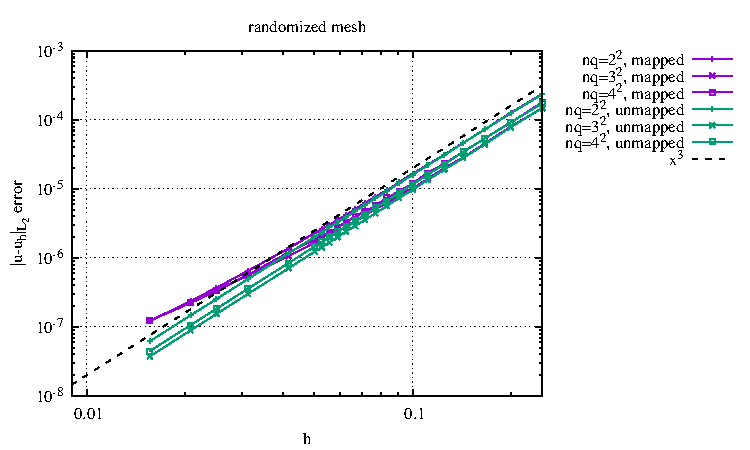
\includegraphics[width=5.7cm]{python_codes/fieldstone_76/results/bench3/rand/errors_V}
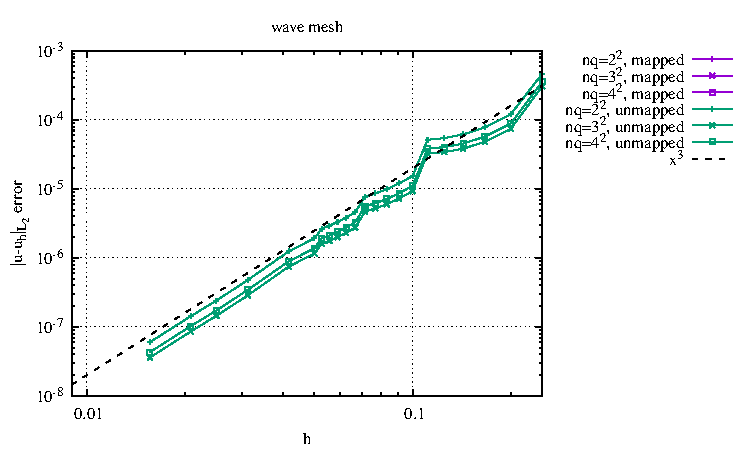
\includegraphics[width=5.7cm]{python_codes/fieldstone_76/results/bench3/wave/errors_V}\\
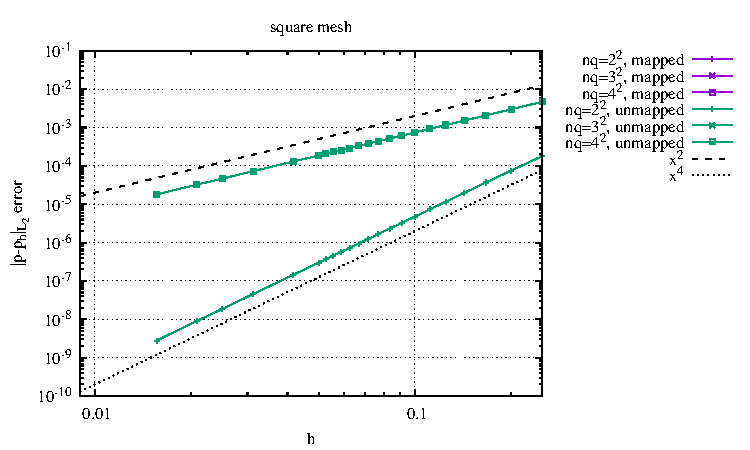
\includegraphics[width=5.7cm]{python_codes/fieldstone_76/results/bench3/reg/errors_P}
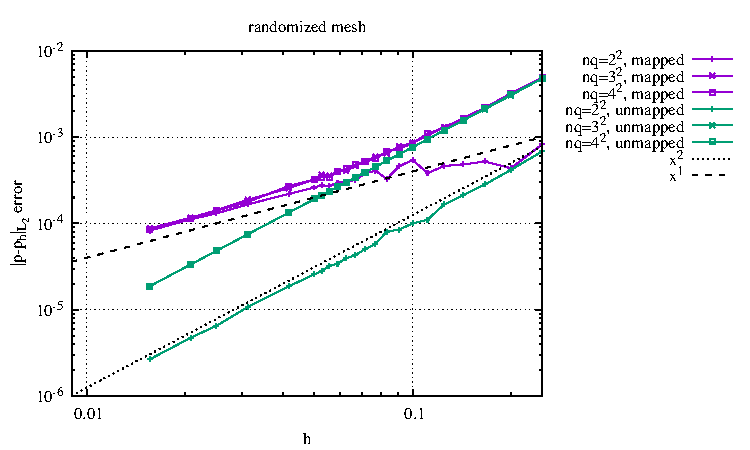
\includegraphics[width=5.7cm]{python_codes/fieldstone_76/results/bench3/rand/errors_P}
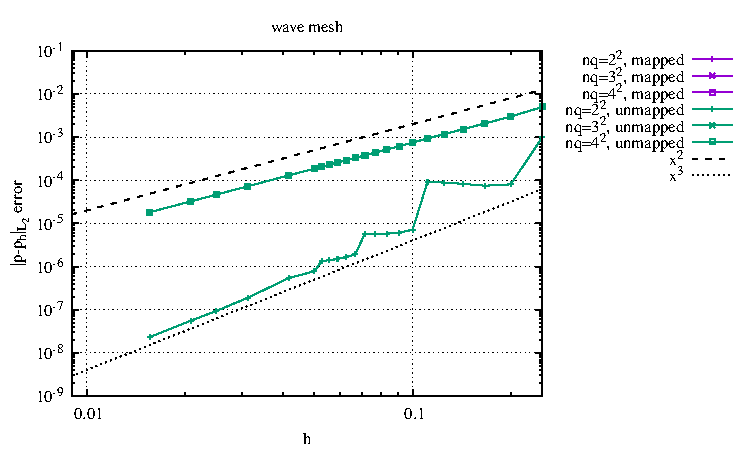
\includegraphics[width=5.7cm]{python_codes/fieldstone_76/results/bench3/wave/errors_P}\\
{\captionfont Left column: Regular square mesh; middle column: Randomized $\xi=0.1$ mesh;
right column: wave mesh.}
\end{center}

This is rather peculiar. I seem to recover 
a 4th order convergence for the pressure error on the square meshes when 
$2\times 2$ quadratures are used but not higher order ones...? 
This does not happen with either randomised meshes or 
other manufactured solutions so I will attribute this superconvergence 
to a combination of facts, i.e. the pressure field is independent 
of $y$ and is only a second order polynomial in $x$, 
terms are under-integrated and elements are all square. 

This observation is no more true on random or wave meshes. 
On random meshes the velocity error convergence rate becomes less than 3 
at high(er) resolutions and the pressure error convergence rate is 1
for the mapped approach and 2 for the un-mapped. 
Note that in the latter case higher order quadratures $3^2$ and $4^2$ yield pressure errors
that are about an order of magnitude higher than those obtained with $2^2$ 
quadratures (again, an unexpected result).

Looking at the results obtained on wave meshes, we see that there is no difference between 
mapped and un-mapped. Furthermore higher order quadratures $3^2$ and $4^2$ yield pressure errors rates 
of 4 while the rate obtained with $2^2$ is 3.

All in all, some of these results are somewhat surprising, but they can be attributed to 
a combination of specific factors.

Let us now consider two other manufactured solutions which showcase a pressure field 
that is a function of $x^m$ and $y^n$ where $m,n\ge 1$.



\newpage
%......................................................
\subsection*{Manufactured solution \#1 ({\tt bench=1})}

The analytical solution originates in Lamichhane (2017) \cite{lami17}.
The velocity and pressure are given by
\begin{eqnarray}
u(x,y)&=&-2x^2y(2y-1)(x-1)^2(y-1) \\
v(x,y)&=& 2xy^2(2x-1)(x-1)(y-1)^2 \\
p(x,y)&=& x(1-x)(1-2y)
\end{eqnarray}
Boundary conditions are no-slip on all sides of the unit square. 
The corresponding body force terms are derived in Section~\ref{MMM-ss:mms11}. 

\begin{center}
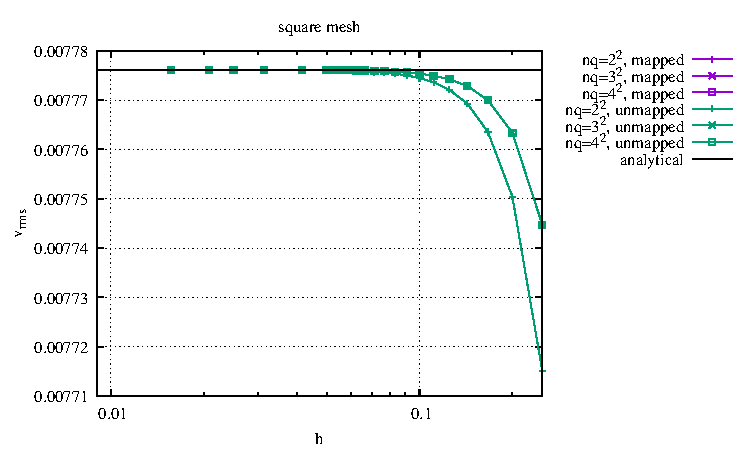
\includegraphics[width=5.7cm]{python_codes/fieldstone_76/results/bench1/reg/vrms}
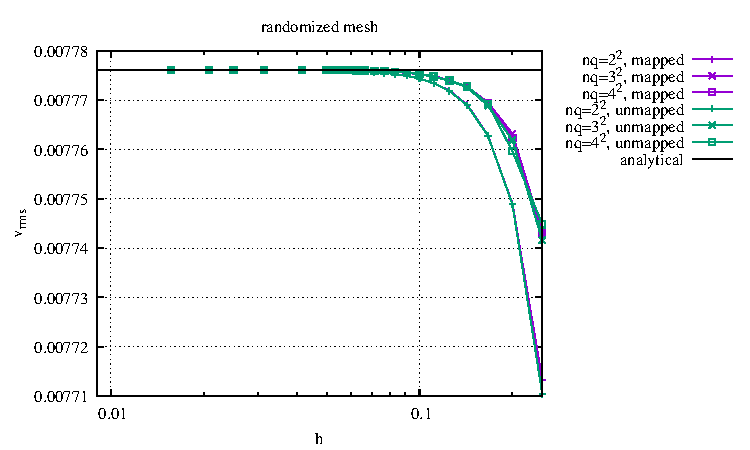
\includegraphics[width=5.7cm]{python_codes/fieldstone_76/results/bench1/rand/vrms}
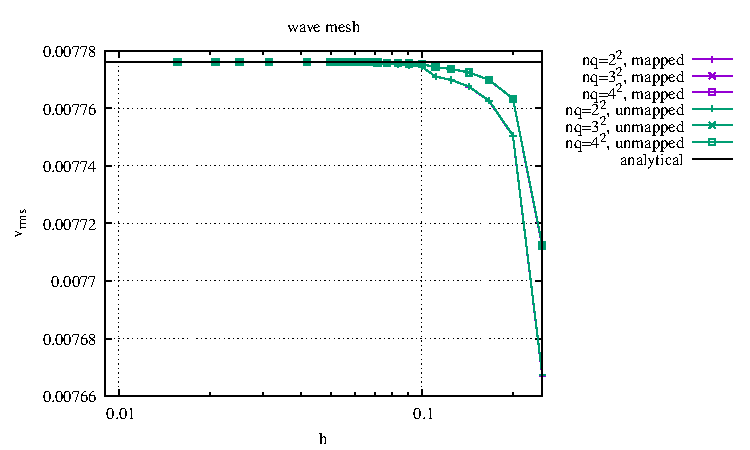
\includegraphics[width=5.7cm]{python_codes/fieldstone_76/results/bench1/wave/vrms}\\
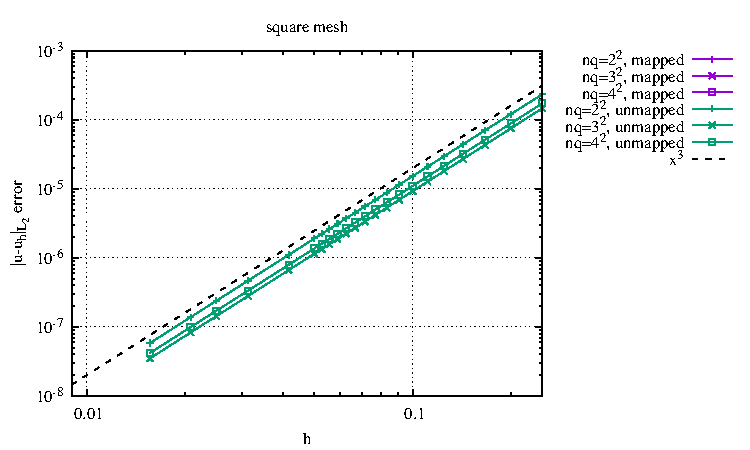
\includegraphics[width=5.7cm]{python_codes/fieldstone_76/results/bench1/reg/errors_V}
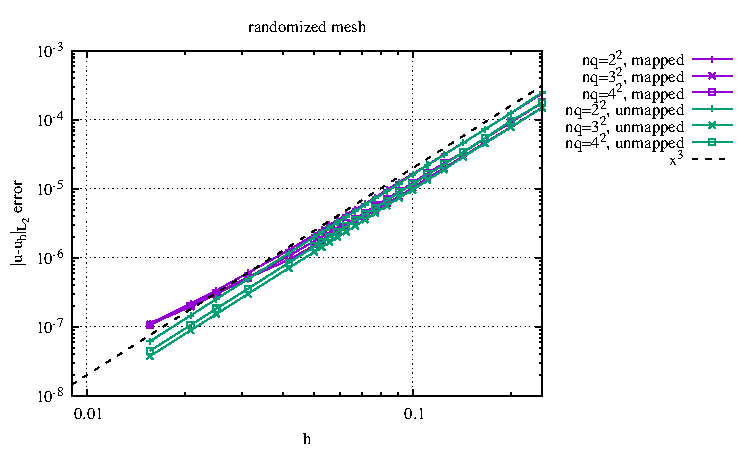
\includegraphics[width=5.7cm]{python_codes/fieldstone_76/results/bench1/rand/errors_V}
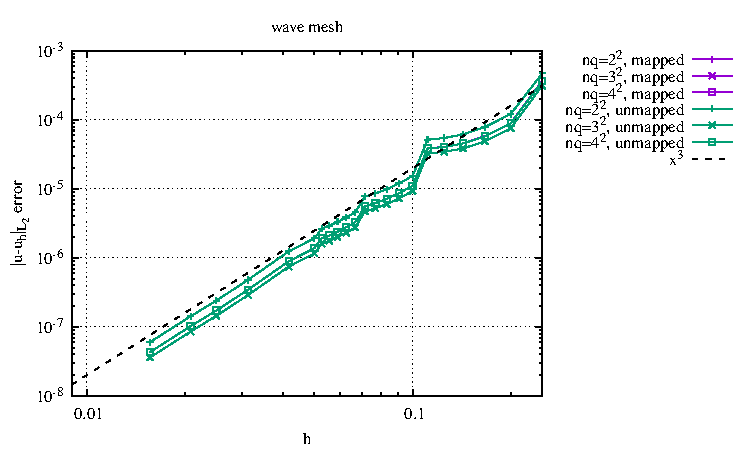
\includegraphics[width=5.7cm]{python_codes/fieldstone_76/results/bench1/wave/errors_V}\\
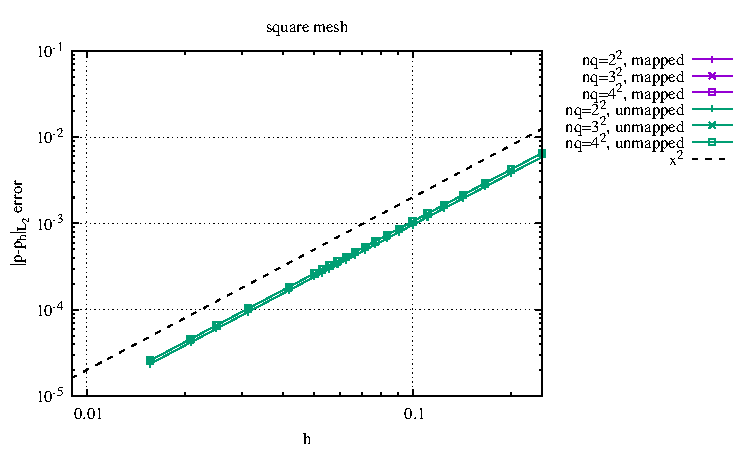
\includegraphics[width=5.7cm]{python_codes/fieldstone_76/results/bench1/reg/errors_P}
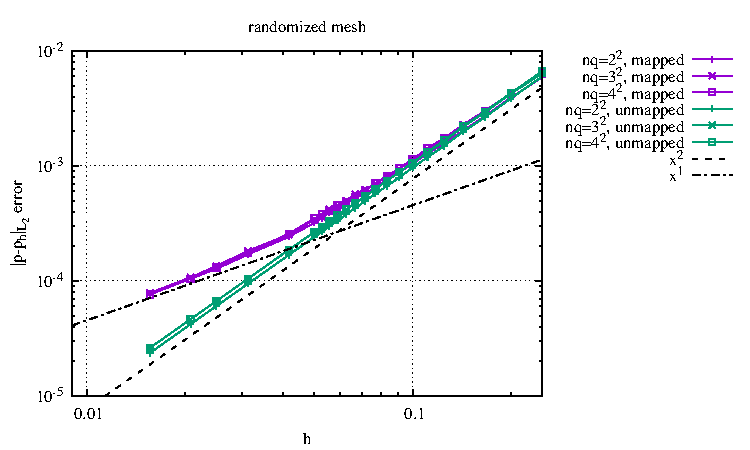
\includegraphics[width=5.7cm]{python_codes/fieldstone_76/results/bench1/rand/errors_P}
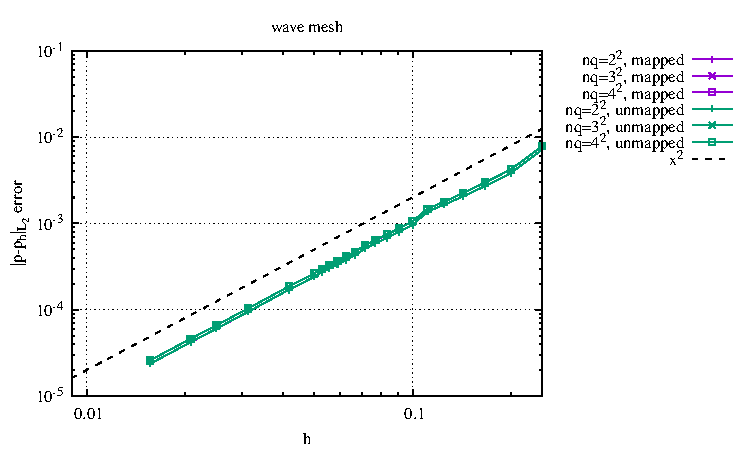
\includegraphics[width=5.7cm]{python_codes/fieldstone_76/results/bench1/wave/errors_P}\\
{\captionfont Left column: Regular square mesh; middle column: Randomized $\xi=0.1$ mesh;
right column: wave mesh.}
\end{center}

The picture in this case is much clearer than before. 
For square and wave meshes the velocity errors and pressure errors
converge with rates 3 and 2 respectively and there is 
no difference between mapped and un-mapped results. Quadrature also does not 
play any role.

In the case of the random meshes pressure error convergence rates are 1 for mapped and 
2 for un-mapped.


\newpage
%......................................................
\subsection*{Manufactured solution \#2 ({\tt bench=9})}

This is the second manufactured solution 
mentioned in Lamichhane \cite{lami17}. It is presented in Section~\ref{MMM-ss:mms2}.
It is for a unit square with $\eta=1$ and the smooth exact solution is
\begin{eqnarray}
u(x,y) &=& x+x^2 - 2xy+x^3 - 3xy^2 + x^2y \\
v(x,y) &=& -y-2xy+y^2 -3x^2y + y^3 - xy^2 \\
p(x,y) &=& xy+x+y+x^3y^2 - 4/3
\end{eqnarray}
Note that the pressure obeys $\int_{\Omega} p \; dV = 0$. The analytical 
velocity is prescribed on the boundary of the domain. 

\begin{center}
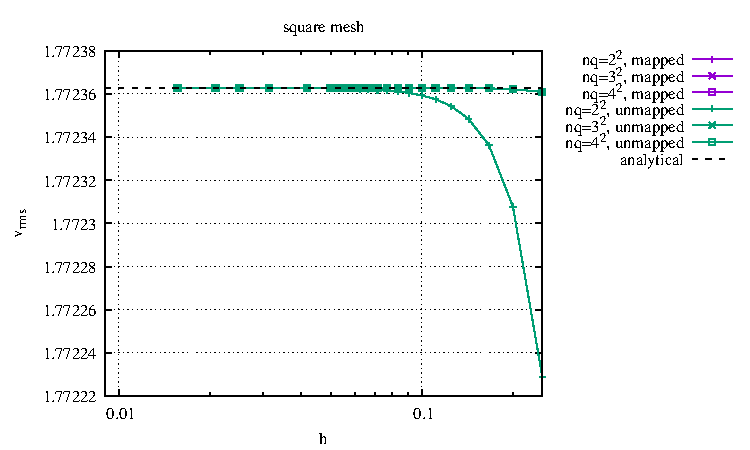
\includegraphics[width=5.7cm]{python_codes/fieldstone_76/results/bench9/reg/vrms}
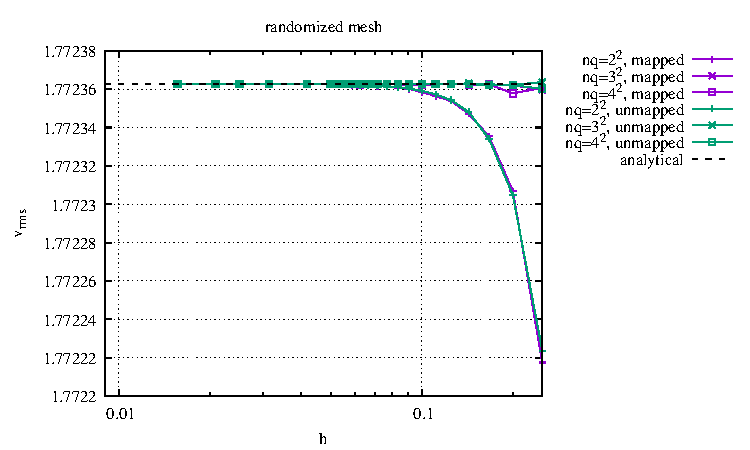
\includegraphics[width=5.7cm]{python_codes/fieldstone_76/results/bench9/rand/vrms}
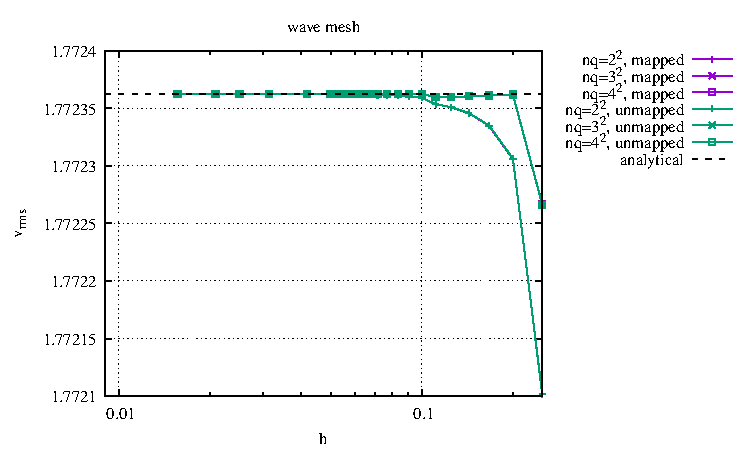
\includegraphics[width=5.7cm]{python_codes/fieldstone_76/results/bench9/wave/vrms}\\
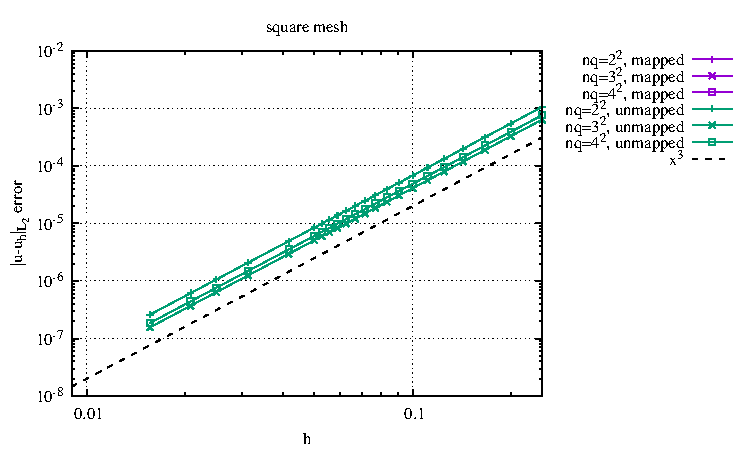
\includegraphics[width=5.7cm]{python_codes/fieldstone_76/results/bench9/reg/errors_V}
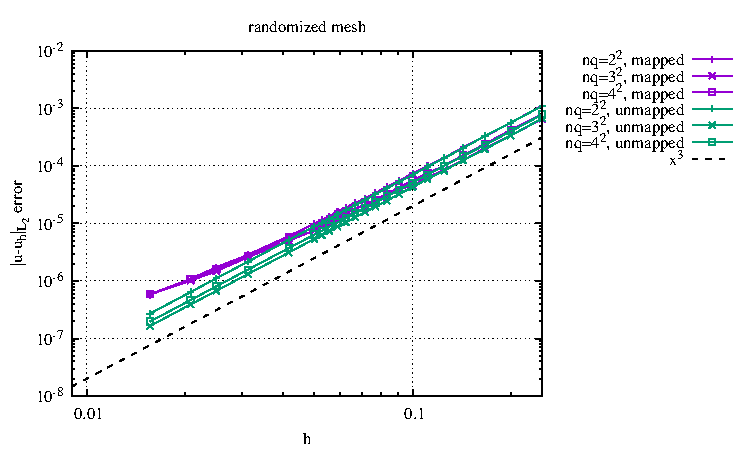
\includegraphics[width=5.7cm]{python_codes/fieldstone_76/results/bench9/rand/errors_V}
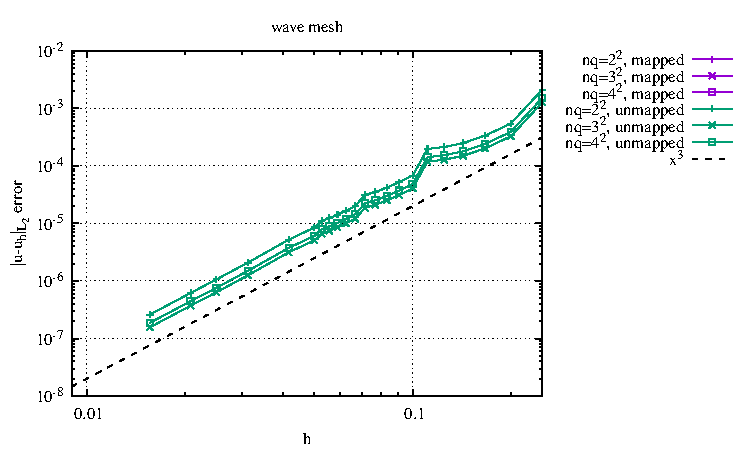
\includegraphics[width=5.7cm]{python_codes/fieldstone_76/results/bench9/wave/errors_V}\\
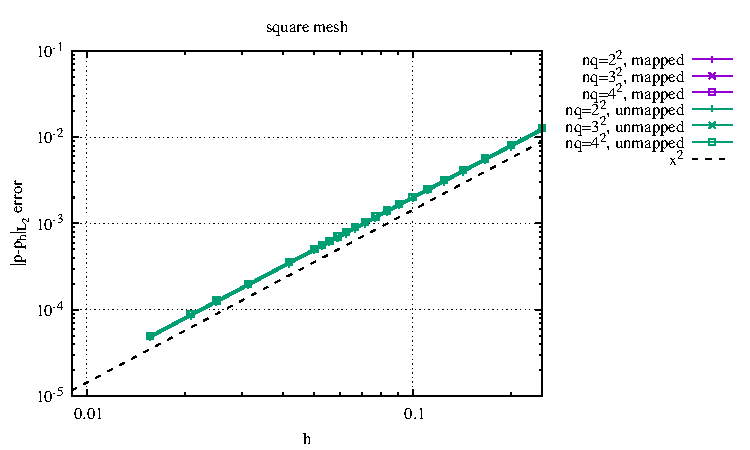
\includegraphics[width=5.7cm]{python_codes/fieldstone_76/results/bench9/reg/errors_P}
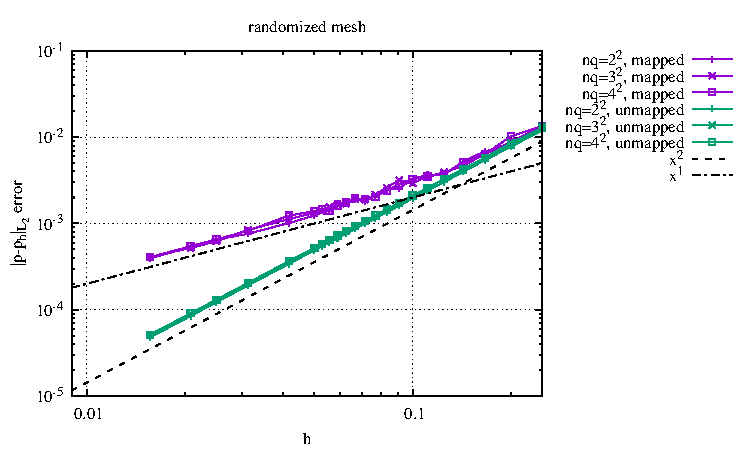
\includegraphics[width=5.7cm]{python_codes/fieldstone_76/results/bench9/rand/errors_P}
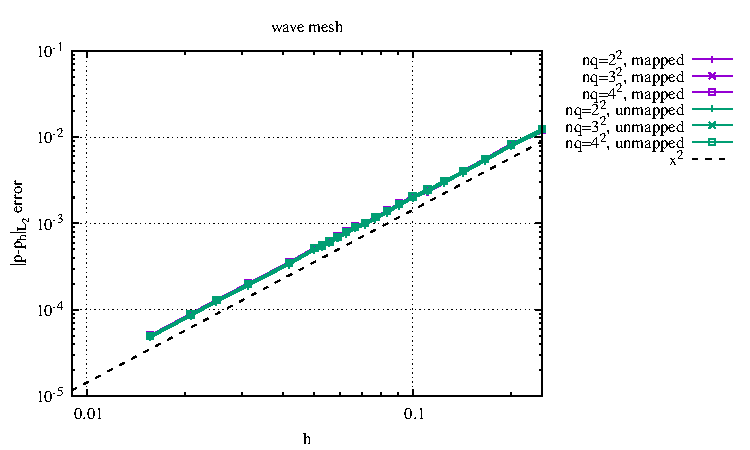
\includegraphics[width=5.7cm]{python_codes/fieldstone_76/results/bench9/wave/errors_P}\\
{\captionfont Left column: Regular square mesh; middle column: Randomized $\xi=0.1$ mesh;
right column: wave mesh.}
\end{center}

We can draw the same conclusions here as for the previous manufactured solution.  


\newpage
%.......................................................
\subsection*{Instantaneous sinking block}

It is fully described in Section~\ref{MMM-ss:sinking_block}.
The block is centered in the domain, its density is 1\% larger than the 
fluid density ($\rho_f=1$) and its viscosity is 1000 times larger than 
the fluid viscosity ($\eta_f=1$).
The block is a square of dimension 1/8 so that using square meshes $16^2$, 
$32^2$, $48^2$, $64^2$, ... ensures that element edges align with the 
sides of the block.
Free-slip boundary conditions are prescribed on all sides.
This is not a benchmark {\it stricto sensu} as there is no analytical solution
available. 

\begin{center}
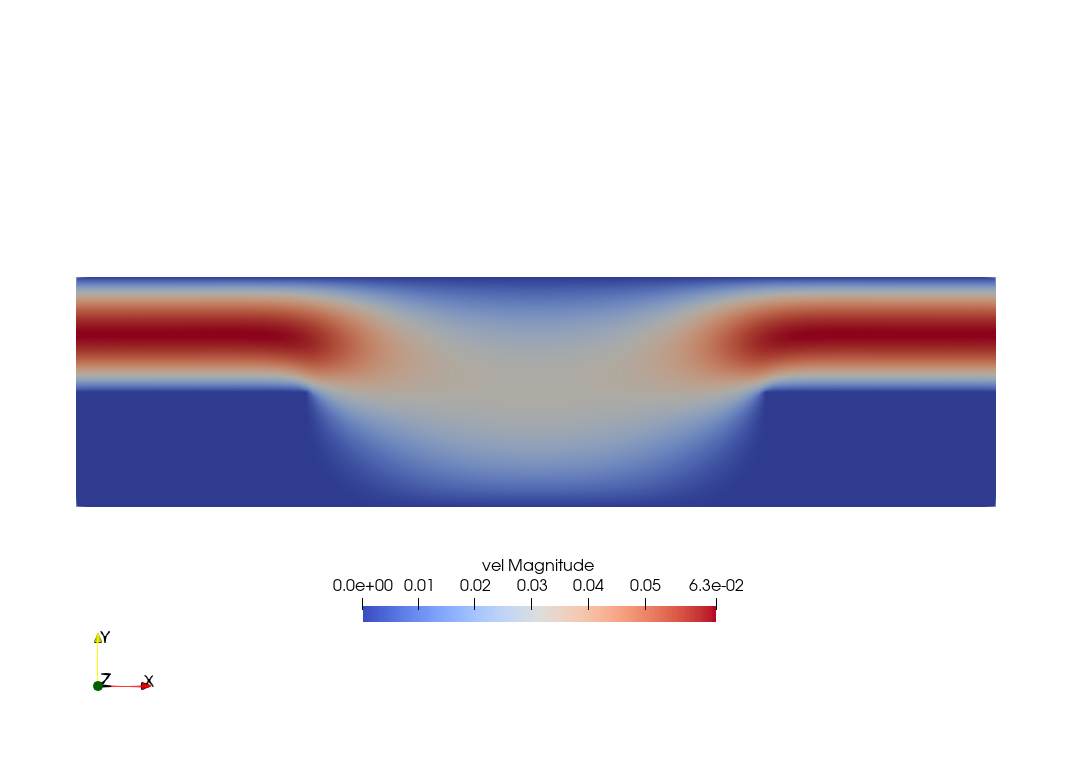
\includegraphics[width=5cm]{python_codes/fieldstone_76/results/block/vel}
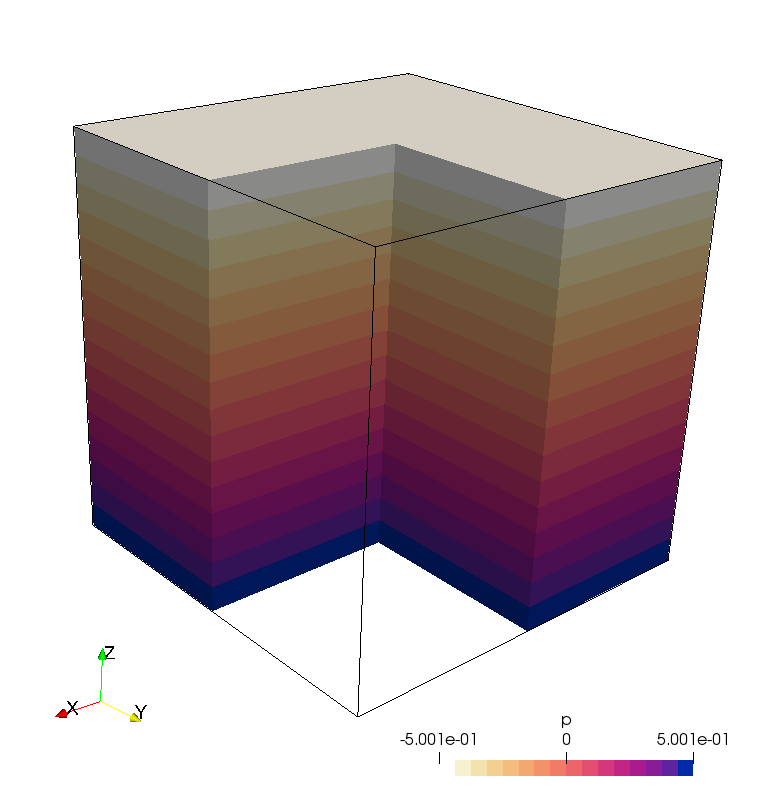
\includegraphics[width=5cm]{python_codes/fieldstone_76/results/block/press}\\
{\captionfont Velocity and pressure fields.}
\end{center}

The root mean square velocity is measured on a series of meshes 
and is shown on the following figure for both mapped and un-mapped approaches: 

\begin{center}
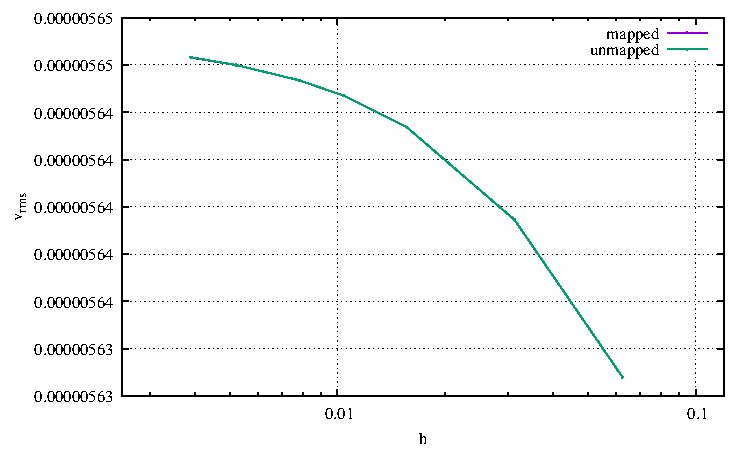
\includegraphics[width=6cm]{python_codes/fieldstone_76/results/block/vrms.pdf}
\end{center}

We find that the highest resolution $80^2$ is not high enough to yield a resolution-independent
measurement (although we note that the measurements above do not vary by more than 1\%). 

The velocity and pressure are measured on a vertical line passing through the 
middle of the block:

\begin{center}
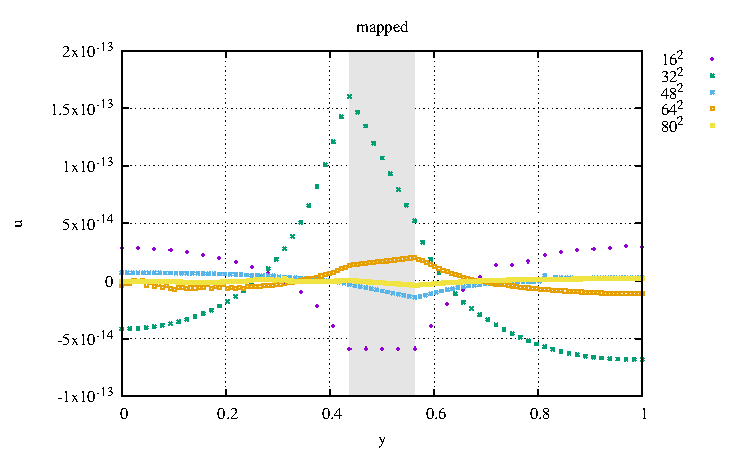
\includegraphics[width=5.7cm]{python_codes/fieldstone_76/results/block/profile_m1_u.pdf}
\includegraphics[width=5.7cm]{python_codes/fieldstone_76/results/block/profile_m1_v.pdf}
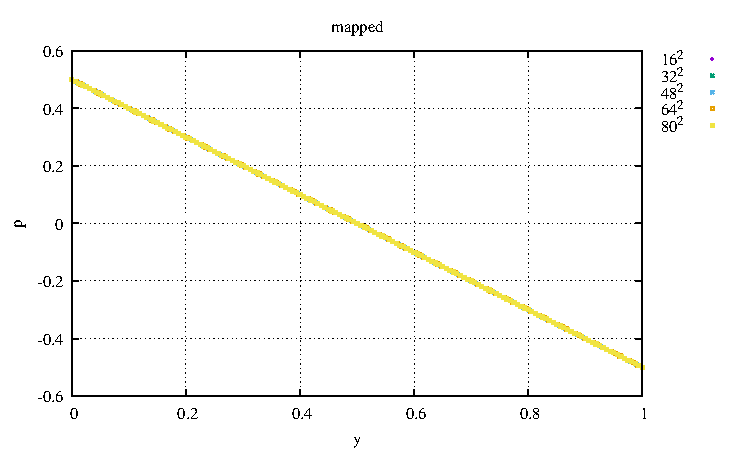
\includegraphics[width=5.7cm]{python_codes/fieldstone_76/results/block/profile_m1_p.pdf}\\
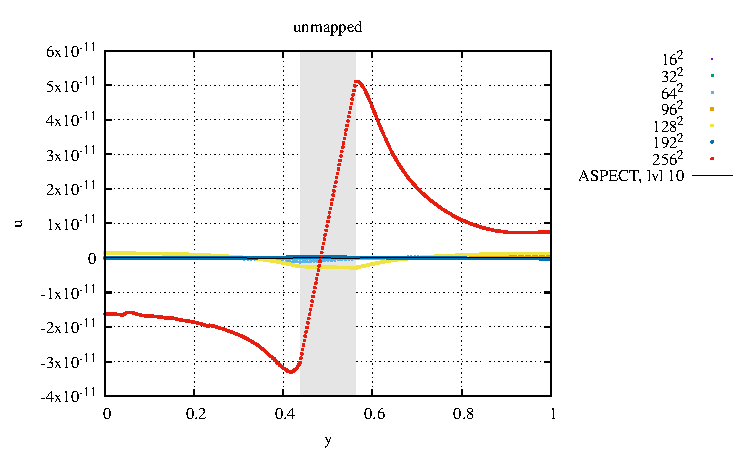
\includegraphics[width=5.7cm]{python_codes/fieldstone_76/results/block/profile_m2_u.pdf}
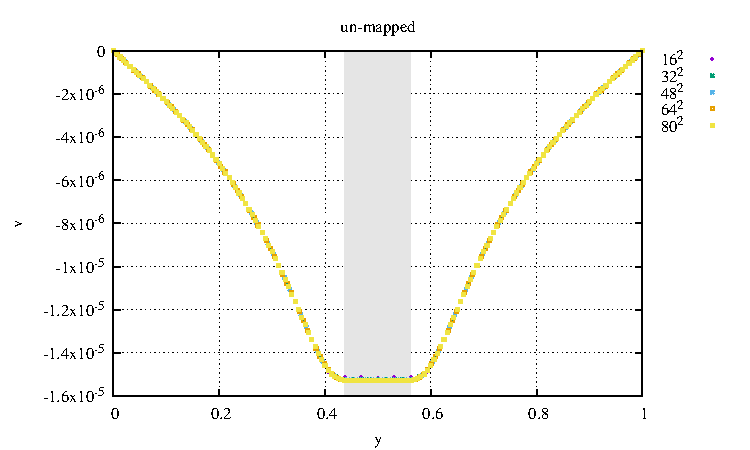
\includegraphics[width=5.7cm]{python_codes/fieldstone_76/results/block/profile_m2_v.pdf}
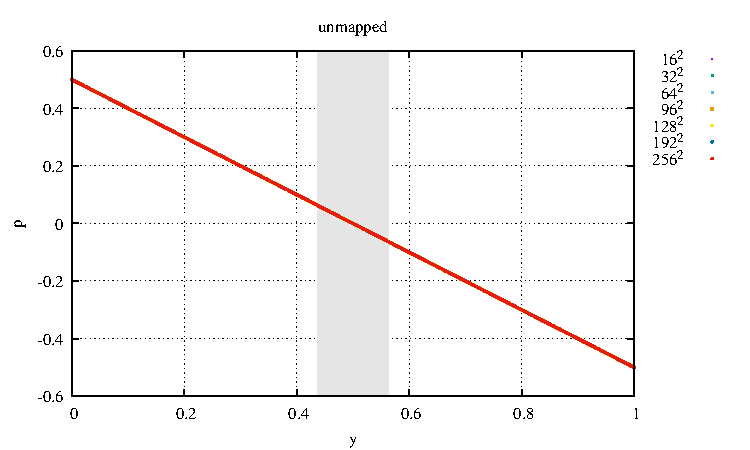
\includegraphics[width=5.7cm]{python_codes/fieldstone_76/results/block/profile_m2_p.pdf}\\
{\captionfont The grey band indicates the $y$ values inside the block.}
\end{center}

Because of symmetry we expect and recover $u=0$ on this line.
The $v$-component seems to converge to a resolution independent profile
while the pressure is clearly dominated by the hydrostatic pressure.
We do not observe any difference between mapped and un-mapped, as expected
since elements are square.

\newpage
%............................................................
\subsection*{Instantaneous sinking block (reduced densities)}

The setup is identical to the previous one, except that now the fluid density is zero and 
the block density is 0.01. In other words the hydrostatic pressure has been removed.
We expect an identical velocity field but the recovered pressure is now the 
dynamic/excess pressure:

\begin{center}
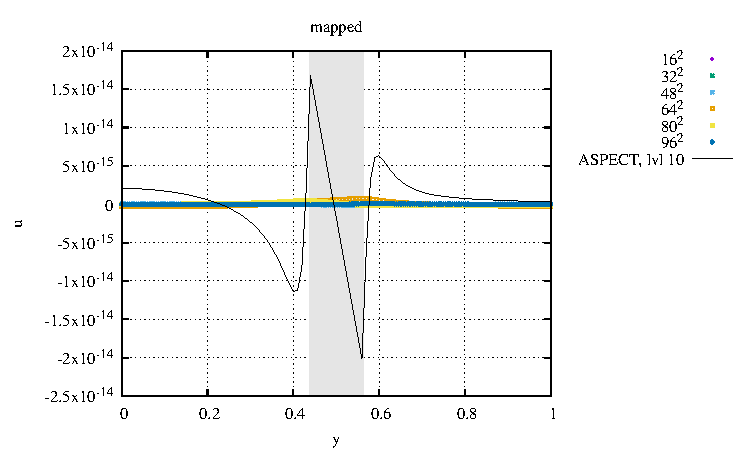
\includegraphics[width=5.7cm]{python_codes/fieldstone_76/results/block_rd/profile_m1_u.pdf}
\includegraphics[width=5.7cm]{python_codes/fieldstone_76/results/block_rd/profile_m1_v.pdf}
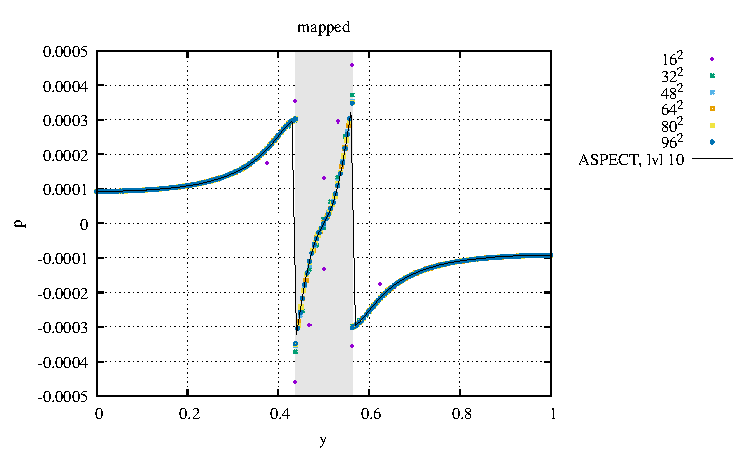
\includegraphics[width=5.7cm]{python_codes/fieldstone_76/results/block_rd/profile_m1_p.pdf}\\
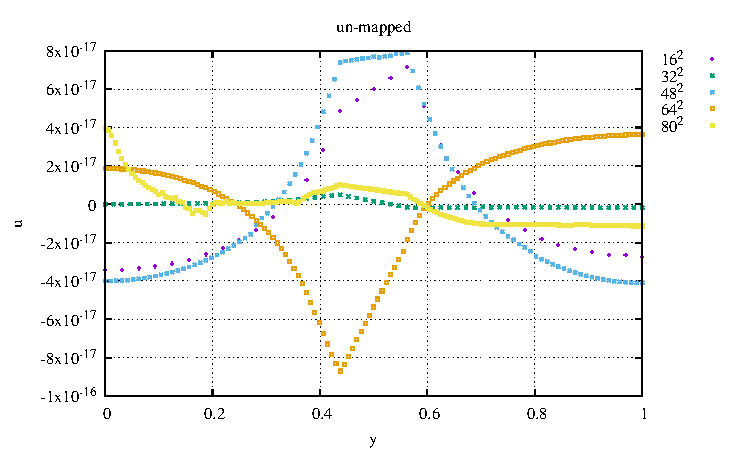
\includegraphics[width=5.7cm]{python_codes/fieldstone_76/results/block_rd/profile_m2_u.pdf}
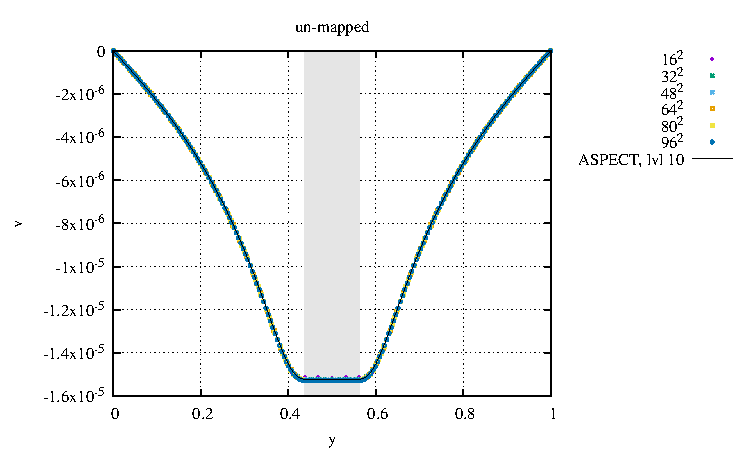
\includegraphics[width=5.7cm]{python_codes/fieldstone_76/results/block_rd/profile_m2_v.pdf}
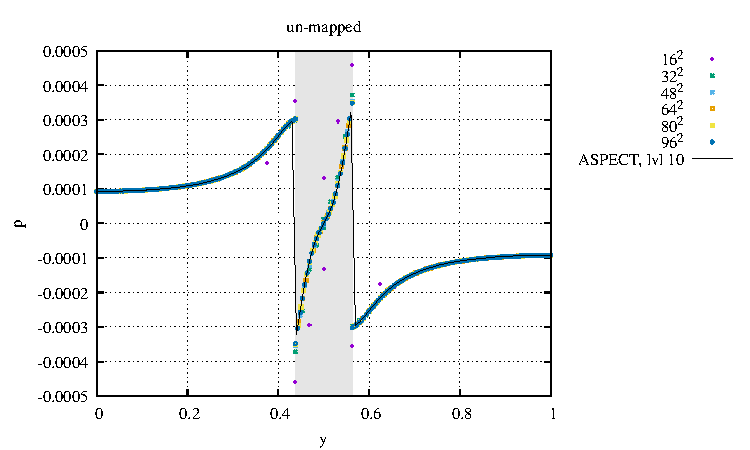
\includegraphics[width=5.7cm]{python_codes/fieldstone_76/results/block_rd/profile_m2_p.pdf}\\
{\captionfont The grey band indicates the $y$ values inside the block.}
\end{center}

We find that results obtained with ASPECT nicely agree with the results of this \stone.

\begin{center}
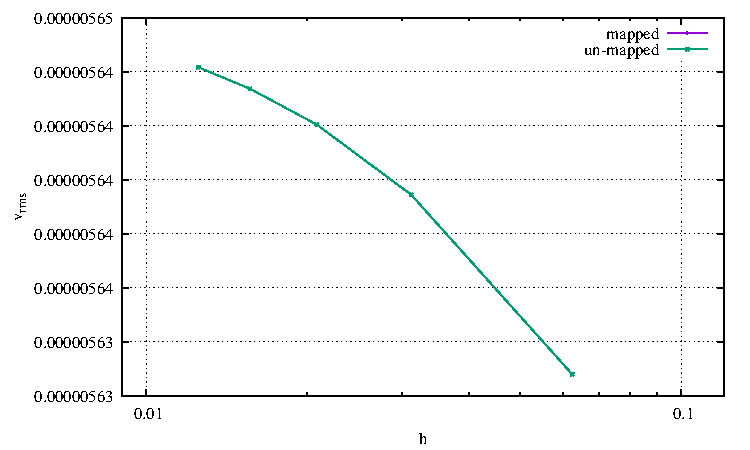
\includegraphics[width=8cm]{python_codes/fieldstone_76/results/block_rd/vrms.pdf}
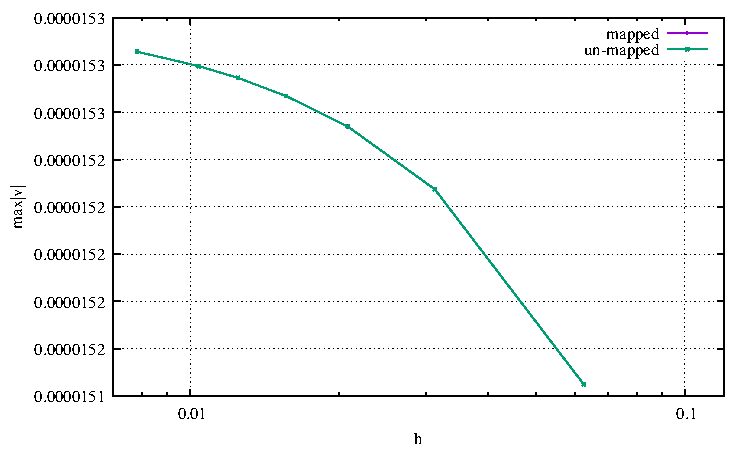
\includegraphics[width=8cm]{python_codes/fieldstone_76/results/block_rd/maxvel.pdf}
\end{center}

\begin{center}
\includegraphics[width=5.7cm]{python_codes/fieldstone_76/results/block_rd/u}
\includegraphics[width=5.7cm]{python_codes/fieldstone_76/results/block_rd/v}
\includegraphics[width=5.7cm]{python_codes/fieldstone_76/results/block_rd/press}\\
{\captionfont Velocity and pressure fields on $96\times 96$ mesh. 
Note that the visualised pressure is elemental instead of $P_{-1}$.}
\end{center}




